\documentclass[a4paper,12pt]{article}

\usepackage[
    left=2cm,
    right=2cm,
    top=3cm,
    bottom=3cm
]{geometry}

\usepackage[utf8]{inputenc}
\usepackage[czech]{babel}
\usepackage[T1]{fontenc}
\usepackage{graphicx}
\usepackage{array}
\usepackage{booktabs}
\usepackage{tabularx}
\usepackage{makecell}
\usepackage{float}
\usepackage{newunicodechar}
\usepackage{url}
\usepackage{siunitx}
\usepackage{listings}
\usepackage{xcolor}
\usepackage{diagbox}
\usepackage{hyperref}
\usepackage{tikz}
\usepackage{pgfplots}
\pgfplotsset{compat=1.18}

\usepackage{fancyhdr}
\pagestyle{fancy}

\fancyhf{}
\fancyhead[L]{SME -- Lab 6: Senzory el. proudu, měření výkonu}
\fancyhead[R]{Pavel Pernička}
\fancyfoot[C]{\thepage}

\fancypagestyle{firstpage}{
    \fancyhf{}
    \renewcommand{\headrulewidth}{0pt}
    \renewcommand{\footrulewidth}{0pt}
    \fancyfoot[C]{\thepage}
}

\definecolor{myblue}{RGB}{111,0,248}
\newcommand{\colorcircle}[1]{%
  \tikz[baseline=-0.6ex]\draw[fill=#1,draw=none] (0,0) circle (1.5ex);%
}
\newcommand{\unitC}{\,^\circ\mathrm{C}}
\newcommand{\unitV}{\,\mathrm{V}}
\newcommand{\unitA}{\,\mathrm{A}}
\newcommand{\units}{\,\mathrm{s}}
\newcommand{\unitmin}{\,\mathrm{min}}

\newcommand{\centered}[1]{\begin{tabular}{l} #1 \end{tabular}}

\addto\captionsczech{\renewcommand{\refname}{Seznam použité literatury}}
\addto\captionsczech{\renewcommand{\figurename}{\textbf{Obrázek}}}
\addto\captionsczech{\renewcommand{\tablename}{\textbf{Tabulka}}}
\renewcommand{\lstlistingname}{\textbf{Kód}}

\lstset{
    language=Python,
    basicstyle=\ttfamily\footnotesize,
    keywordstyle=\color{blue},
    commentstyle=\color{gray},
    stringstyle=\color{red},
    numbers=left,
    numberstyle=\tiny\color{gray},
    stepnumber=1,
    breaklines=true,
    frame=single
}

\begin{document}
\thispagestyle{firstpage}

\vspace*{\fill}
\begin{center}
\renewcommand{\arraystretch}{1.75}

\begin{tabularx}{\textwidth}{|X|X|X|}
    \hline
    \multicolumn{1}{|c|}{\rule{0pt}{2.25cm} 
\includegraphics[height=2cm]{img/ctu_logo.png}}
    & \multicolumn{2}{c|}{\makecell{\textbf{KATEDRA MĚŘENÍ}}} \\
    \hline
    \multicolumn{3}{|c|}{\Large \textbf{\centered{Senzory a měření}}} \\
    \hline
    \multicolumn{2}{|X}{\small{Jméno} \newline \textbf{Pavel Pernička}}
    & \multicolumn{1}{|X|}{\small{Datum měření} \newline \textbf{11.3.2026}} \\
    \hline
    {\small{Semestr} \newline \textbf{Letní 2026}}
    & {\small{Ročník} \newline \textbf{2.}}
    & {\small{Datum odevzdání} \newline \textbf{18.3.2026}} \\
    \hline
    \multicolumn{3}{|c|}{\rule{0pt}{1cm}} \\
    \hline
    \multicolumn{1}{|X|}{\small{Číslo úlohy \newline \textbf{6}}}
    & \multicolumn{2}{|p{9cm}|}{\small{Název úlohy \newline \textbf{Senzory el. proudu, měření výkonu}}} \\
    \hline
\end{tabularx}

\end{center}
\vspace*{\fill}

\newpage
\pagestyle{fancy}
\section{Domácí příprava}
\begin{itemize}
  \item Jaký je rozdíl mezi napěťovým a proudovým transformátorem?
    \begin{itemize}
      \item Proudový transformátor se používá k měření proudu vodičem. Ten vodič je prostrčený skrz jádro transformátoru a slouží jako primární vinutí. Proud měříme jakožto napětí na rezistoru, který je připojen na sekundární vinutí.
      \item Napěťový transformátor slouží k převodu vyššího/nižšího napětí podle poměru závitů na primárním a sekundárním vinutí.
    \end{itemize}
  \item Uveďte typy proudových senzorů, které umožňují měřit stejnosměrný proud popř. střídavý proud včetně stejnosměrné složky. Který z nich je galvanicky oddělený?
    \begin{itemize}
      \item Hallův senzor -- měří magnetickou indukci, je galvanicky oddělený
      \item Proudový bočník -- není galvanicky oddělený
      \item Magnetorezistivní senzory -- jsou galvanicky oddělené
    \end{itemize}
  \item Jaký senzor proudu (převodník proud-napětí) je použit v případě 1a) a 1b)?
    \begin{itemize}
      \item Proudový bočník. V případě 1a) zabudovaný přímo v multimetru, v případě 1b) je externí.
    \end{itemize}
  \item Jaký senzor proudu (převodník proud-napětí) je použit v případě 1c)?
    \begin{itemize}
      \item Proudový transformátor s rezistorem na sekundárním vinutí.
    \end{itemize}
  \item Vysvětlete pojem „Insertion impedance“ používaný u sensorů pracujících na magnetickém principu.
    \begin{itemize}
      \item Impedance, kterou senzor ovlivňuje proud v měřeném obvodu.
    \end{itemize}
  \item Jaké jsou výhody a nevýhody kompenzovaného a nekompenzovaného proudového senzoru s Hallovou sondou?
    \begin{itemize}
      \item Nekompenzovaný senzor -- prostě Hallův senzor v blízkosti vodiče. Výhoda je jednoduchost a cena, nevýhody jsou herší přesnost, nelinearita, teplotní drift
      \item Kompenzovaný senzor -- výstup halova senzoru jde so další sekundární cívky na transformůtoru, kde zpětnou vazbou nuluje magnetický tok. Druhým sekundárním vinutím měříme proud pomocí napětí na rezistoru na něm. Výhody jsou linearita a~přesnost, nevýhodou je nutnost mít dva sekundáry a více elektroniky.
    \end{itemize}
  \item Jakým způsobem lze zvýšit citlivost proudového transformátoru nebo proudových kleští?
    \begin{itemize}
      \item Více závitů, lepší jádro transformátoru, větší rezistor
    \end{itemize}
  \item Připomeňte si z fyziky Ampérův zákon – jak se v této úloze uplatňuje?
    \begin{itemize}
      \item Magnetické pole v jádře je úměrné proudu procházejícího vodičem
    \end{itemize}
\end{itemize}

\section{Měření}
\subsection{Proud jednofázovou zátěží změřený několika přístroji}
Změřte proud tekoucí jednofázovou zátěží následujícími přístroji/senzory:

\subsubsection{Ručním multimetrem s interním bočníkem}
\begin{itemize}
  \item Přístroj: \textbf{Summit 45}
  \item Odpor přístroje: \textbf{malý (bočník)}
  \item Přesnost: $(\pm 1,5 \%\ + 3\ \mathrm{digity})$
  \item Hodnota proudu v případě:
    \begin{itemize}
      \item Harmonický průběh proudu: efektivní hodnota (měří střední hodnotu, ale je kalibrovaný na sinusový průběh)
      \item Neharmonický průběh proudu: změří nepřesně
      \item Přítomnost DC složky: V DC režimu ji změříme docela přesně, v AC režimu ji nevidíme (kondenzátor na vstupu).
    \end{itemize}
  \item Naměřeno: $\mathbf{I_1 = 2{,}448\ A}$
  \item Nejistota měření:
  $$
    \Delta I_1 = \pm \left(0{,}015 \cdot 2{,}448 + 0{,}003\right)
    = \pm \left(0{,}03672 + 0{,}003\right)\ \mathrm{A}
    = \pm 0{,}03972\ \mathrm{A}.
  $$
  \item Výsledek: $\mathbf{I_1 = (2{,}448 \pm 0{,}040)\ \mathrm{A}}$
\end{itemize}

\subsubsection{Pomocí externího bočníku a milivoltmetru}
\begin{itemize}
  \item Přístroj: \textbf{HP 34401A + bočník HP 34330A $1mV/A$}
  \item Odpor bočníku: $1\ m\Omega$
  \item Přesnost voltmetru: $(\pm 0,012 \%\ + 3\ \mathrm{digity})$
  \item Přesnost bočníku: $0,3\ \%$ do frekvence $1\ kHz$
  \item Hodnota proudu v případě:
    \begin{itemize}
      \item Harmonický průběh proudu: True RMS
      \item Neharmonický průběh proudu: True RMS
      \item Přítomnost DC složky: v AC režimu ne, v DC režimu ano
    \end{itemize}
  \item Naměřeno: $\mathbf{I_2 = 2{,}478\ A}$
  \item Nejistota měření:

  $$
    I = \frac{U}{R_s}
  $$

  $$
    u_C(I) = \sqrt{
      \left( \frac{\partial I}{\partial U} \cdot u(U) \right)^2 +
      \left( \frac{\partial I}{\partial R_s} \cdot u(R_s) \right)^2
    }
  $$

  $$
    \frac{\partial I}{\partial U} = \frac{1}{R_s} = \frac{1}{0{,}001} = 1000
  $$

  $$
    \frac{\partial I}{\partial R_s} = -\frac{U}{R_s^2}
    = -\frac{0{,}002478}{0{,}001^2}
    = -2478
  $$

  $$
    u(U) = \frac{0{,}00012 \cdot 0{,}002478 + 3 \cdot 10^{-6}}{\sqrt{3}}
    = \frac{0{,}000003297}{\sqrt{3}}\ \mathrm{V}
  $$

  $$
    u(R_s) = \frac{0{,}003 \cdot 0{,}001}{\sqrt{3}} = \frac{0{,}000003}{\sqrt{3}}\ \Omega
  $$

  $$
    u_C(I_2) = \sqrt{(1{,}90 \cdot 10^{-6})^2 +(4{,}29 \cdot 10^{-6})^2} \approx 4{,}7 \cdot 10^{-6}\ \mathrm{A}.
  $$

  \item Výsledek: $\mathbf{I_2 = (2{,}478 \pm 0{,}008)\ \mathrm{A}}$
\end{itemize}

\subsubsection{Proudovým transformátorem}
\begin{itemize}
  \item Přístroj: \textbf{MXD-4660A + proud. transformátor (1:2500)}
  \item Přesnost voltmetru: $(\pm 0,5 \%\ + 10\ \mathrm{digit})$
  \item Rezistor na sekundáru: $10\ \Omega, 0,1\ \%$
  \item Hodnota proudu v případě:
    \begin{itemize}
      \item Harmonický průběh proudu: efektivní hodnota
      \item Neharmonický průběh proudu: závisí na spektru
      \item Přítomnost DC složky: neměříme
    \end{itemize}
  \item Naměřeno: $U_3 = 9{,}78\ \mathrm{mV} \Rightarrow \mathbf{I_3 = 2{,}445\ \mathrm{A}}$
  \item Nejistota měření:

  $$
    I = \frac{nU}{R}
  $$

  $$
    u_C(I) = \sqrt{
      \left( \frac{\partial I}{\partial U} \cdot u(U) \right)^2 +
      \left( \frac{\partial I}{\partial R} \cdot u(R) \right)^2
    }
  $$

  $$
    \frac{\partial I}{\partial U} = \frac{n}{R} = \frac{2500}{10} = 250\
  $$

  $$
    \frac{\partial I}{\partial R} = -\frac{nU}{R^2}
    = -\frac{2500 \cdot 0{,}00978}{10^2}
    = -0{,}2445
  $$

  $$
    u(U) = \frac{0{,}005 \cdot 0{,}00978 + 10 \cdot 0{,}00001}{\sqrt{3}}
    = \frac{0{,}0001489}{\sqrt{3}}\ \mathrm{V}
  $$

  $$
    u(R) = \frac{0{,}001 \cdot 10}{\sqrt{3}} = \frac{0{,}01}{\sqrt{3}}\ \Omega
  $$

  $$
    u_C(I_3) = \sqrt{(250 \cdot 8{,}59 \cdot 10^{-5})^2 + (0{,}2445 \cdot 5{,}77 \cdot 10^{-3})^2},\approx 0{,}0216\ \mathrm{A}.
  $$

  \item Výsledek: $\mathbf{I_3 = (2{,}445 \pm 0{,}021)\ \mathrm{A}}$
\end{itemize}

\subsubsection{Klešťovým ampérmetrem – wattmetrem}
\begin{itemize}
  \item Přístroj: \textbf{Parkside HG06985A}
  \item Odpor přístroje: desítky ohmů (nevidíme vnitřní realizaci přístroje)
  \item Přesnost: $(\pm 4 \%\ + 15\ \mathrm{digity})$
  \item Hodnota proudu v případě:
    \begin{itemize}
      \item Harmonický průběh proudu: True RMS
      \item Neharmonický průběh proudu: závisí na spektru
      \item Přítomnost DC složky: neměříme
    \end{itemize}
  \item Naměřeno: $I_m = 7{,}30\ \mathrm{A}$ (3 závity) $\Rightarrow \mathbf{I_4 = 2{,}43\ \mathrm{A}}$
  \item Nejistota měření:

  $$
    \Delta I_m = \pm(0{,}04 \cdot 7{,}30 + 15 \cdot 0{,}01)
    = \pm(0{,}292 + 0{,}15)
    = \pm 0{,}442\ \mathrm{A}
  $$

  $$
    U_B(I_4) = \frac{0{,}442}{3\cdot \sqrt{3}} \approx 0{,}085\ \mathrm{A}
  $$

  \item Výsledek: $\mathbf{I_4 = (2{,}43 \pm 0{,}08)\ \mathrm{A}}$
\end{itemize}

\subsubsection{Pomocí proudových kleští a osciloskopu}
\begin{itemize}
  \item Přístroj: \textbf{osciloskop + kleště HP1146A}
  \item Insertion impedance: $10\ m\Omega$
  \item Přesnost: $4\ \%$
  \item Hodnota proudu v případě:
    \begin{itemize}
      \item Harmonický průběh proudu: Vidíme průběh (zde bereme efektivní hodnotu)
      \item Neharmonický průběh proudu: Vidíme průběh
      \item Přítomnost DC složky: Kleště jsou založeny na Hallově sondě, DC složka by měla být měřitelná
    \end{itemize}
  \item Naměřeno: $\mathbf{I_5 = 2,4640\ A}$ (pomocí Masurements, viz obrázek \ref{fig:oscilak})
\end{itemize}

\begin{figure}[H]
\centering
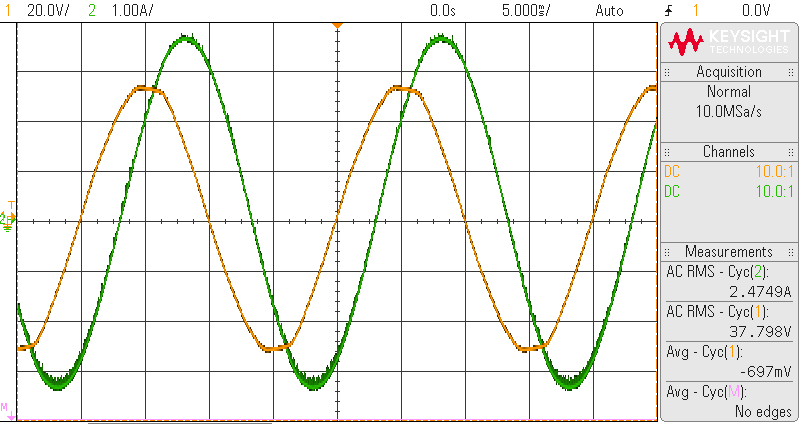
\includegraphics[width=0.90\textwidth]{img/scope.png}
\caption{Snímek průběhu na osciloskopu se zapojenými kleštěmi}
\label{fig:oscilak}
\end{figure}

\subsection{Analyzátor výkonu Tektronix PA1000}
Naměřili jsme příkon $P=59,4\ W$, power factor $\cos \varphi = 0,536$. Průběh napětí, proudu a~výkonu je zobrazen na obrázku \ref{fig:anal} vyexportovaném z obslužného programu.

\begin{figure}[H]
\centering
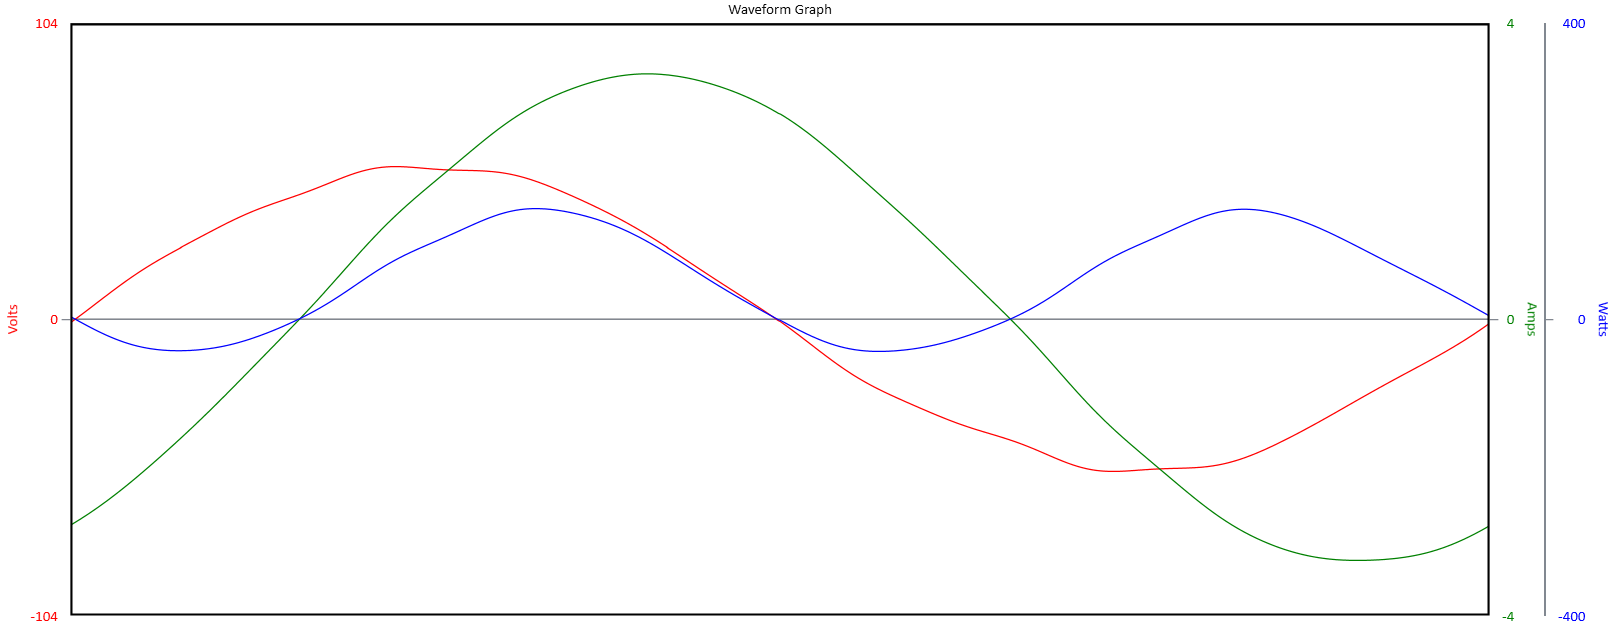
\includegraphics[width=0.90\textwidth]{img/analyzer.png}
\caption{Snímek obrazovky softwaru PWRVIEW}
\label{fig:anal}
\end{figure}

\subsection{Elektroměr}
Ten naměřil proud $I_6 = 2,46\ A$, příkon $P = 51\ W$, při napětí $U = 37,8\ V$. Tyto údaje jsou poměrmě dost blízko naměřeným hodnotám pomocí jiných přístrojů.

\end{document}
